% This file was adapted from ICLR2022_conference.tex example provided for the ICLR conference
\documentclass{article} % For LaTeX2e
\usepackage{conference,times}
\usepackage{easyReview}
\usepackage{algorithm}
\usepackage{algorithmic}

% Optional math commands from https://github.com/goodfeli/dlbook_notation.
\input{math_commands.tex}

\usepackage{amsthm,amssymb}

\newtheorem{theorem}{Theorem}[section]
\newtheorem{corollary}{Corollary}[theorem]
\newtheorem{lemma}[theorem]{Lemma}
\newtheorem{definition}[theorem]{Definition}

% Please leave these options as they are
\usepackage{hyperref}
\hypersetup{
    colorlinks=true,
    linkcolor=red,
    filecolor=magenta,
    urlcolor=blue,
    citecolor=purple,
    pdftitle={Inner-Shell Raman X-Gate Tradeoffs in Neutral Yb-171},
    pdfpagemode=FullScreen,
    }



\title{Inner-Shell Raman X-Gate Tradeoffs for a Neutral $^{171}$Yb Nuclear Qubit at Fixed Optical Power}

\author{Marius-Constantin Dinu \\
Independent Research \\
\texttt{marius.constantin.dinu@proton.me}}

\begin{document}


\maketitle

\begin{abstract}
We study single-qubit $X$-gate feasibility for a $^{171}$Yb nuclear-spin qubit encoded in the $^3P_0(F=1/2)$ manifold and driven by Raman coupling through an inner-shell-excited $J=2$ intermediate. The design objective is explicitly constrained: optical intensity is fixed at $1\,\mathrm{W/cm^2}$, and the output must report gate-time versus target-infidelity operating points at $10^{-2}$, $10^{-3}$, $10^{-4}$, and $10^{-5}$. We develop a hybrid formal-empirical methodology that combines (i) a convex surrogate optimality certificate for detuning selection, (ii) a robust feasibility-floor certificate for impossibility regions, and (iii) a posterior chance-constrained table for uncertainty-aware decision support. The resulting evidence indicates a stable, non-provisional operating regime at $10^{-2}$ with a best deterministic gate time of $0.1661\,\mu\mathrm{s}$ and dominant leakage contribution. After targeted posterior uncertainty ablations (model-discrepancy and noise-floor scaling), posterior confidence intervals widen materially and strict-threshold recommendations at $10^{-3}$ and below become infeasible in both deterministic and posterior modules. Those strict rows remain provisional because robust-floor diagnostics still classify $10^{-3}$ as potentially feasible under conservative assumptions. Beyond this specific gate, the study connects atomic-structure uncertainty management to broader neutral-atom processor planning and high-accuracy metrology workflows.
\end{abstract}

\section{Introduction}
Neutral-atom quantum hardware is now transitioning from proof-of-principle control demonstrations to operating regimes where model fidelity, uncertainty accounting, and architecture-aware calibration are first-order constraints rather than post hoc corrections \citep{S08,S13,S14,S15}. In alkaline-earth-like systems, ytterbium is an especially interesting platform because precision spectroscopy, long-lived clock states, and neutral-atom array engineering can be integrated in one physical stack \citep{S02,S03,S04,S07,S17,S20,S21}. This dual role creates an opportunity and a risk: the same weakly allowed transitions that make ultra-stable metrology possible can also introduce difficult control tradeoffs when repurposed for fast quantum gates.

The concrete problem here is intentionally narrow. We consider an $X$ gate on a $^{171}$Yb qubit encoded in the two-state $^3P_0(F=1/2)$ manifold, with Raman transfer through an inner-shell-excited $4f^{13}5d6s^2(J=2)$ intermediate. Optical power is fixed at $1\,\mathrm{W/cm^2}$, and performance must be summarized at target infidelities $10^{-2}$ through $10^{-5}$. This setting is motivated by the scientific attractiveness of inner-shell Yb transitions \citep{S01,S02,S06} and by the practical need to determine whether strict targets are genuinely reachable under realistic uncertainty in matrix elements, branching ratios, and calibration noise.

Existing work provides crucial building blocks but no direct answer to this specific constrained question. Raman scattering analyses provide mechanistic scaling relations \citep{S11,S12}, clock-systematic literature clarifies the nontrivial role of probe and Stark shifts \citep{S09,S10,S16}, and neutral-atom benchmarking literature clarifies plausible fidelity bands in adjacent hardware contexts \citep{S13,S14,S15}. However, there is still a methodological gap between these ingredients and a gate-design decision rule that simultaneously reports speed, feasibility, uncertainty, and formal validity conditions for the same operating envelope.

This manuscript fills that gap using a hybrid pipeline that combines theorem-backed structure with simulation-backed evidence. We do not claim final physical constants for every inner-shell channel; instead, we make the uncertainty explicit, derive what can be certified under those assumptions, and isolate where conclusions remain provisional. This framing is useful both for quantum-computing decisions and for cross-domain experimental planning in precision spectroscopy and system identification.

Our main contributions are:
\begin{itemize}
\item We formulate a constrained Yb-specific Raman $X$-gate optimization problem that explicitly couples scattering, leakage, Stark, and control terms under a fixed-intensity feasibility set.
\item We prove a unique interior optimum for a convex surrogate detuning model and show how that certificate can be used to generate thresholded fastest-feasible candidates.
\item We derive a robust impossibility-floor criterion that cleanly separates feasible from infeasible target regions under conservative channel-wise lower bounds.
\item We integrate deterministic and posterior chance-constrained analyses into one tradeoff report, exposing where conclusions are strong and where they remain provisional due to uncertainty-model limitations.
\end{itemize}

The manuscript is intentionally written as a decision artifact rather than a best-case performance narrative. In practical hardware planning, a recommendation is only useful when the assumptions that justify it are visible, when failure modes are explicit, and when downstream experiments can be prioritized using concrete acceptance criteria. For that reason, each major claim in this paper is paired with a theorem, a table, a figure, or a combination of those elements, and the strongest and weakest confidence regimes are separated explicitly instead of being averaged into a single headline number. This style is relevant outside the immediate Yb setting: uncertainty-aware claim promotion is equally important in fault-tolerance planning, high-accuracy spectroscopy deployment, and architecture-level resource allocation where optimistic but brittle estimates can misdirect entire development cycles.

\Secref{sec:related} situates this work in prior literature, \secref{sec:setting} defines the formal problem and notation, \secref{sec:methods} presents the method and formal statements, \secref{sec:results} reports quantitative findings with claim-to-evidence links, and \secref{sec:discussion} details limitations and follow-up experiments needed to close remaining gaps.

\section{Related Work and Gap Analysis}
\label{sec:related}
\subsection{Inner-Shell Yb Transition Context}
The inner-shell $J=2$ transition in neutral Yb has moved from theory-driven plausibility to direct experimental accessibility over the last several years. Atomic-structure and sensitivity analyses identified the transition family as potentially long-lived and high-value for precision tests \citep{S01,S06}. Subsequent observations established experimentally resolved spectroscopy, including hyperfine and Zeeman structure needed for realistic control discussions \citep{S02,S03,S04}. This sequence is important because the gate-design question depends on both classes of evidence: theory alone cannot bound implementation losses, and spectroscopy alone does not yield operating-time versus error tradeoff surfaces.

A strength of this body of work is high physical specificity for ytterbium. A limitation is that most publications optimize for clock performance or fundamental-physics sensitivity, not for fastest constrained qubit-gate synthesis under fixed optical intensity. As a result, relevant constants exist, but the target decision variable is different.

\subsection{Raman Error Models and Transferability}
Raman scattering analyses provide the most reusable analytic structure for speed-versus-fidelity tradeoffs. Foundational trapped-ion analyses show how spontaneous scattering floors emerge from detuning, linewidth, and level-structure scales \citep{S11}, and later refinements show where simple formulas can be conservative \citep{S12}. These models are a strength because they expose explicit parametric dependence and support theorem-level manipulations.

Their limitation in this context is transferability. The inner-shell Yb pathway is not numerically identical to the canonical trapped-ion settings used to derive baseline formulas. Consequently, direct parameter substitution can be misleading unless uncertainty propagation is carried through all terms and feasibility claims are explicitly conditioned on that uncertainty.

\subsection{Shift Suppression and Noise-Coupling Literature}
Clock-control literature has established that pulse engineering can suppress probe-induced shifts dramatically in idealized conditions \citep{S09}. However, intensity fluctuations and correlated noise can reintroduce bias and narrow the practical robustness margin \citep{S10}. Modern lattice-shift studies reinforce that calibration quality and environmental stability can dominate once obvious first-order error channels are reduced \citep{S16}. For weakly allowed pathways, quadrupole-coupling analyses further show that geometry and polarization structure can materially change effective interaction strength, which motivates explicit feasibility constraints in our setting \citep{S05}.

The strength of this line is methodological realism: it emphasizes that the best nominal solution is not automatically the most reliable one. The limitation is that these protocols are not typically framed as thresholded gate-time decision tables across multiple infidelity targets with explicit feasibility flags.

\subsection{Neutral-Atom Performance Benchmarks and System Context}
Recent neutral-atom results provide a trajectory of improved gate fidelity and larger operational scale \citep{S13,S14,S15,S20,S21}. These works are essential for context: they bound what is plausible in adjacent architectures and motivate why aggressive thresholds such as $10^{-4}$ and $10^{-5}$ are scientifically meaningful. They also show that Yb-specific control and calibration pipelines can support universal gate primitives in optical-tweezer arrays \citep{S22}. Related excited-state control studies in trapped-ion platforms provide additional cautionary analogs for coherence-sensitive operating regions \citep{S18,S19}.

At the same time, mechanism mismatch remains a limitation for direct transfer. Rydberg-mediated entangling gate achievements and architecture-level scaling results do not directly resolve the specific inner-shell Raman single-qubit tradeoff considered here. Hence, benchmark context should constrain priors and expectations, not replace mechanism-faithful modeling.

\subsection{Recent Yb-Focused Control and Simulation Signals}
Recent preprints provide additional directional evidence on where inner-shell Raman studies may evolve, although these reports should be interpreted as context rather than finalized constants. Dual-encoding Yb designs suggest that combining optical and hyperfine manifolds can expand control flexibility while preserving long coherence windows \citep{S23}. Work on electric-field-error mitigation and coherent-error suppression in programmable arrays similarly indicates that calibration architecture, not only pulse algebra, will likely dominate strict-threshold reliability in advanced regimes \citep{S25,S29}. High-fidelity single-qubit gate reports in neutral-atom settings further reinforce that single-qubit performance can approach demanding targets when hardware and calibration pipelines are co-designed \citep{S34}.

These sources are useful because they highlight practical levers that are absent from purely analytic formulations: field compensation, model-discrepancy handling, and calibration workflow design. They are limited because most are preprint-stage and not mechanism-identical to an inner-shell Raman $X$ gate in $^{171}$Yb. We therefore use them as hypothesis-shaping context, not as primary numeric evidence for the thresholded table.

Scalable simulation methodology is another relevant axis. Efficient large-array simulation and uncertainty-propagation proposals suggest how this single-gate analysis can be embedded into broader system-level optimization once parameter identifiability improves \citep{S27}. Updated atomic-data compendia also indicate a path to reducing uncertainty in matrix-element priors, but those updates still require cross-validation against mechanism-specific spectroscopy before strict-threshold gate claims can be promoted without reservation \citep{S24}.

\subsection{Gap Motivating This Manuscript}
Taken together, prior work gives: (i) strong Yb transition motivation \citep{S01,S02,S06}, (ii) reusable Raman error physics \citep{S11,S12}, (iii) robust-shift caution \citep{S09,S10,S16}, and (iv) platform-level performance direction \citep{S13,S14,S15,S20,S21}. Missing is a unified, uncertainty-explicit decision framework that, under fixed intensity and a fixed Raman mechanism, reports thresholded gate-time tradeoffs together with formal statements about optimality and infeasibility boundaries. This manuscript addresses that missing layer.

\section{Problem Setting, Symbols, and Objectives}
\label{sec:setting}
\subsection{State Space and Control Space}
We consider computational basis states $\{|0\rangle,|1\rangle\}$ encoded in the two-level $^3P_0(F=1/2)$ manifold of $^{171}$Yb. Raman coupling proceeds through an inner-shell intermediate state manifold denoted $|e\rangle$ associated with the $J=2$ branch. The control variable is
\begin{equation}
\vu = (\Delta,\phi) \in \mathcal{U},
\label{eq:control}
\end{equation}
where $\Delta$ is one-photon detuning and $\phi$ indexes pulse family and phase schedule. The feasible control set is
\begin{equation}
\mathcal{F}=\left\{\vu\in\mathcal{U}: I=1\,\mathrm{W/cm^2},\; \Delta\in[\Delta_{\min},\Delta_{\max}],\; \phi\in\Phi_{\mathrm{hw}}\right\},
\label{eq:feasible}
\end{equation}
with $\Phi_{\mathrm{hw}}$ denoting hardware-admissible pulse shapes.

\subsection{Error Decomposition and Gate-Time Model}
Total infidelity is decomposed as
\begin{equation}
\epsilon_{\mathrm{tot}}(\vu)=\epsilon_{\mathrm{sc}}(\Delta)+\epsilon_{\mathrm{leak}}(\Delta)+\epsilon_{\mathrm{Stark}}(\vu)+\epsilon_{\mathrm{ctrl}}(\vu),
\label{eq:eps_total}
\end{equation}
where the four terms denote scattering, off-manifold leakage, differential Stark/systematic bias, and control-noise contributions, respectively. Gate time is modeled via the effective two-photon coupling,
\begin{equation}
t_{\pi}(\vu)=\frac{\pi}{\Omega_{\mathrm{eff}}(\Delta,\phi)}.
\label{eq:gate_time}
\end{equation}

For each infidelity threshold $\tau\in\{10^{-2},10^{-3},10^{-4},10^{-5}\}$, the speed objective is
\begin{equation}
T_{\tau}^{\star}=\inf_{\vu\in\mathcal{F}}\left\{t_{\pi}(\vu):\epsilon_{\mathrm{tot}}(\vu)\le\tau\right\}.
\label{eq:threshold_objective}
\end{equation}
This objective explicitly distinguishes two failure modes: infeasibility (no feasible control satisfies the threshold) versus feasibility with high uncertainty.

\subsection{Notation Summary}
Table~\ref{tab:notation} summarizes symbols that recur in \secref{sec:methods} and \secref{sec:results}.

\begin{table}[t]
\caption{Core notation used in the formal model. The table is placed after symbol introduction so each entry links directly to definitions in \secref{sec:setting}.}
\label{tab:notation}
\centering
\small
\renewcommand{\arraystretch}{1.1}
\setlength{\tabcolsep}{4pt}
\begin{tabular}{ll}
\hline
Symbol & Meaning \\
\hline
$\vu=(\Delta,\phi)$ & Control variable: detuning and pulse family parameters \\
$\mathcal{F}$ & Feasible control set at fixed intensity and hardware bounds \\
$\epsilon_{\mathrm{tot}}$ & Total gate infidelity from additive channel decomposition \\
$t_{\pi}$ & Gate duration for a nominal $X(\pi)$ rotation \\
$\tau$ & Target infidelity threshold \\
$T_{\tau}^{\star}$ & Fastest feasible gate time at threshold $\tau$ \\
$\underline{\epsilon}_{\mathrm{floor}}$ & Conservative robust lower bound on achievable infidelity \\
$\alpha$ & Allowed violation probability in chance constraints \\
\hline
\end{tabular}
\end{table}

\subsection{Assumption Ledger and Scope Boundaries}
The scope is intentionally constrained to avoid hidden degrees of freedom. First, optical intensity is fixed and not optimized, so all reported speed improvements arise from detuning and pulse-family selection rather than power scaling. Second, control design is restricted to hardware-admissible families, which prevents unattainable pulse shapes from biasing feasibility claims. Third, we treat channel decomposition in \eqref{eq:eps_total} as an operational accounting identity for this study, while acknowledging that higher-order coupling terms may become relevant in future high-precision calibration campaigns.

Uncertainty assumptions are equally explicit. Atomic parameters and noise terms are represented as uncertain quantities with conservative lower bounds used for robust-floor checks and posterior distributions used for chance-constrained decisions. This dual treatment is deliberate: robust bounds answer what cannot be achieved under declared assumptions, while posterior models answer what may be feasible with calibrated risk tolerance. If either assumption family is invalidated by new measurements, corresponding claims must be demoted and re-evaluated.

Finally, the target outputs are decision-facing and thresholded. We do not optimize a single scalar objective across all regimes because that would obscure physically important discontinuities between feasible and infeasible tiers. Instead, each threshold is treated as a separate constrained problem with its own evidence status, which better matches experimental planning where resources are allocated by milestone.

\section{Hybrid Methodology}
\label{sec:methods}
\subsection{Detuning Surrogate and Interior Optimality Certificate}
For fixed pulse family and local operating region, we use $x=\Delta^2>0$ and the surrogate
\begin{equation}
f(x)=\frac{A}{x}+Bx+C, \quad A>0,\;B>0.
\label{eq:surrogate}
\end{equation}
This captures the canonical tradeoff where scattering-like terms decrease with detuning while control penalties increase.

\begin{theorem}[Unique interior optimum of the surrogate]
\label{thm:fc1}
Assume $A>0$ and $B>0$ in \eqref{eq:surrogate}. Then $f$ is strictly convex on $(0,\infty)$ and has a unique global minimizer
\begin{equation}
x^{\star}=\sqrt{\frac{A}{B}},\qquad
\Delta^{\star}=\left(\frac{A}{B}\right)^{1/4}.
\label{eq:delta_star}
\end{equation}
\end{theorem}

\begin{proof}
Differentiating \eqref{eq:surrogate} gives $f'(x)=-A/x^2+B$ and $f''(x)=2A/x^3$. Since $A>0$ and $x>0$, we have $f''(x)>0$ for all $x\in(0,\infty)$, so $f$ is strictly convex. The stationary condition $f'(x)=0$ implies $x^2=A/B$ and therefore $x^{\star}=\sqrt{A/B}>0$. Strict convexity guarantees that this stationary point is unique and globally minimizing on $(0,\infty)$. Substituting $x=\Delta^2$ yields \eqref{eq:delta_star}.\qedhere
\end{proof}

\Eqref{eq:delta_star} is used as a candidate generator, not as a stand-alone physical guarantee. Candidate controls are retained only if full model checks satisfy threshold constraints in \eqref{eq:threshold_objective}.

\subsection{Robust Feasibility Floor and Impossibility Statement}
To avoid optimistic over-interpretation, we use conservative lower bounds on irreducible channels:
\begin{equation}
\epsilon_{\mathrm{tot}}(\vu,\rvtheta,\rn)
\ge
\underline{\epsilon}_{\mathrm{sc}}(\rvtheta)+
\underline{\epsilon}_{\mathrm{noise}}(\rn)+
\underline{\epsilon}_{\mathrm{cal}}(\rvtheta)
\equiv
\underline{\epsilon}_{\mathrm{floor}},
\label{eq:floor}
\end{equation}
where $\rvtheta$ denotes uncertain atomic parameters and $\rn$ denotes noise realizations.

\begin{theorem}[Robust infeasibility criterion]
\label{thm:fc2}
If \eqref{eq:floor} holds over the declared uncertainty set and $\underline{\epsilon}_{\mathrm{floor}}>\tau$, then the robust feasible set
\begin{equation}
\mathcal{F}_{\tau}=\left\{\vu\in\mathcal{F}:\epsilon_{\mathrm{tot}}(\vu,\rvtheta,\rn)\le\tau\;\forall (\rvtheta,\rn)\right\}
\label{eq:robust_set}
\end{equation}
is empty.
\end{theorem}

\begin{proof}
Assume by contradiction that $\mathcal{F}_{\tau}$ is non-empty while $\underline{\epsilon}_{\mathrm{floor}}>\tau$. Then there exists $\vu\in\mathcal{F}_{\tau}$ such that $\epsilon_{\mathrm{tot}}(\vu,\rvtheta,\rn)\le\tau$ for every admissible $(\rvtheta,\rn)$. But \eqref{eq:floor} implies $\epsilon_{\mathrm{tot}}(\vu,\rvtheta,\rn)\ge\underline{\epsilon}_{\mathrm{floor}}>\tau$ for those same admissible realizations, contradiction. Therefore $\mathcal{F}_{\tau}=\varnothing$.\qedhere
\end{proof}

This theorem is used to distinguish optimization failure from physical infeasibility: if \eqref{eq:robust_set} is empty, further local search cannot recover the threshold without changing assumptions or resources.

\subsection{Posterior Chance-Constrained Decision Layer}
Deterministic feasibility does not quantify risk under uncertain constants. We therefore add a posterior layer:
\begin{equation}
p(\rvtheta\mid \train)\propto p(\train\mid\rvtheta)p(\rvtheta),
\label{eq:posterior}
\end{equation}
with decision rule
\begin{equation}
T_{\tau}=\inf_{\vu\in\mathcal{F}}\left\{t_{\pi}(\vu):\Pr_{\rvtheta\sim p(\rvtheta\mid\train)}\left[\epsilon_{\mathrm{tot}}(\vu,\rvtheta)\le \tau\right]\ge 1-\alpha\right\}.
\label{eq:chance}
\end{equation}

The role of \eqref{eq:chance} is operational: it returns thresholded speed recommendations with explicit risk tolerance $\alpha$, which can then be compared against deterministic and robust-floor conclusions for consistency.

\subsection{Workflow Overview}
\begin{algorithm}[t]
\caption{Hybrid workflow for thresholded Yb Raman $X$-gate tradeoff synthesis.}
\label{alg:workflow}
\begin{algorithmic}
\STATE Define $\mathcal{F}$ from fixed intensity, detuning window, and hardware pulse limits.
\STATE Fit surrogate coefficients $(A,B,C)$ and verify assumptions $A>0$, $B>0$, and local unimodality.
\STATE Generate interior candidates from \eqref{eq:delta_star} and evaluate full-channel model \eqref{eq:eps_total}.
\STATE Compute robust floor diagnostics via \eqref{eq:floor} and classify infeasible thresholds using Theorem~\ref{thm:fc2}.
\STATE Infer posterior parameters with \eqref{eq:posterior} and solve chance-constrained decisions via \eqref{eq:chance}.
\STATE Merge deterministic, robust, and posterior outputs into one threshold table with provisional flags for conflicts.
\end{algorithmic}
\end{algorithm}

\subsection{Implementation Architecture}
The implementation follows four modules: deterministic sweep and surrogate checks, robust floor stress testing, posterior chance-constrained inference, and integrated consistency aggregation. This modular split is important for scientific traceability: each module has separate acceptance criteria and can fail independently without masking disagreements in the final report. Internal symbolic checks validate the algebra in Theorems~\ref{thm:fc1} and \ref{thm:fc2} before numerical claims are promoted. The numerical implementation strategy is aligned with established open AMO simulation tooling patterns used for reproducibility-oriented parameter studies \citep{S36}.

\subsection{Claim-Promotion Protocol and Falsification Strategy}
The operational sequence in \algref{alg:workflow} defines not only how results are generated but also how claims are promoted or demoted. A claim enters the ``strong'' tier only when three conditions are simultaneously satisfied: (i) theorem assumptions and symbolic checks pass, (ii) empirical diagnostics match acceptance criteria, and (iii) cross-module consistency remains above threshold without unresolved contradictions. If any one of these conditions fails, the claim is marked provisional, even if one module reports favorable nominal performance.

For the detuning-optimum statement, falsification is straightforward: if unimodality or surrogate adequacy fails in accepted runs, Theorem~\ref{thm:fc1} cannot be used as a decision certificate for those regions. For robust-floor statements, falsification requires validated counterexamples where measured or simulated outcomes beat declared conservative floors without violating model assumptions. For posterior statements, falsification occurs when out-of-sample violation rates exceed the declared risk level or when predictive coverage indicates severe miscalibration. This layered falsification design prevents mathematically correct but empirically fragile claims from being over-promoted.

The protocol also separates diagnostic from prescriptive evidence. Diagnostics describe model behavior, while prescriptive evidence supports an actionable operating recommendation. In strict-threshold regimes, diagnostic evidence may remain informative even when prescriptive confidence is insufficient. This distinction matters for efficient follow-up: experiments can be targeted to the exact uncertainty components that block claim promotion, rather than restarting the full analysis pipeline.

\section{Results and Claim-Evidence Alignment}
\label{sec:results}
\subsection{Integrated Tradeoff Outcomes}
Table~\ref{tab:integrated} is the primary decision artifact because it combines deterministic feasibility, robust-floor classification, and posterior risk summaries at the four requested thresholds. The table shows one strong non-provisional regime at $\tau=10^{-2}$ and three provisional rows at stricter targets.

\begin{table*}[t]
\caption{Integrated thresholded tradeoff summary across deterministic, robust-floor, and posterior analyses. The table reports speed, error, feasibility-rate, and consistency diagnostics at each requested target. Provisional flags indicate unresolved methodological disagreement rather than numerical instability in a single module.}
\label{tab:integrated}
\centering
\small
\renewcommand{\arraystretch}{1.1}
\setlength{\tabcolsep}{4pt}
\resizebox{\linewidth}{!}{%
\begin{tabular}{lcccccccc}
\hline
$\tau$ & Deterministic feasible & Best deterministic $t_{\pi}$ ($\mu$s) & Best deterministic $\epsilon_{\mathrm{tot}}$ & Posterior $T_{\tau}$ ($\mu$s) & Posterior violation rate & Robust feasibility rate & Consistency score & Provisional \\
\hline
$10^{-5}$ & No & -- & -- & -- & 1.0 & 0.0 & 0.9433 & Yes \\
$10^{-4}$ & No & -- & -- & -- & 1.0 & 0.0 & 0.9433 & Yes \\
$10^{-3}$ & No & -- & -- & -- & 1.0 & 1.0 & 0.9433 & Yes \\
$10^{-2}$ & Yes & 0.1661 & 0.0061237 & 0.2038 & 4.36e-4 & 1.0 & 0.9433 & No \\
\hline
\end{tabular}}
\end{table*}

The $10^{-2}$ row supports a concrete operating point with deterministic feasibility, robust feasibility, and no cross-module conflict. In contrast, $10^{-3}$ is marked provisional because deterministic and posterior modules now both return no stable feasible candidates after uncertainty ablation, while robust-floor diagnostics still indicate this threshold is not ruled out by conservative lower bounds. That mismatch is the central unresolved issue in the present evidence set.

The integrated table also shows why a single global metric would be misleading. If one optimizes only posterior median gate time, strict targets can appear deceptively attractive unless uncertainty-model stress tests are applied. If one uses only deterministic feasibility, all strict targets collapse into one ``infeasible'' bucket without exposing model-sensitivity structure near $10^{-3}$. By retaining both views in one table and enforcing explicit provisional labels, the analysis preserves decision information that would otherwise be erased by scalarization.

\subsection{Detuning-Structure Evidence for the Interior-Optimum Claim}
\Figref{fig:h1landscape} links directly to Theorem~\ref{thm:fc1}. Panel (a) shows the detuning versus infidelity landscape with uncertainty bands, and panel (b) reports surrogate fit quality across pulse families and prior scales. The observed unimodality pass rate is 1.0 in the executed sweep, which supports the local applicability of the convex surrogate assumptions used to derive \eqref{eq:delta_star}. Under those assumptions, interior candidate generation is justified.

\begin{figure}[t]
\centering
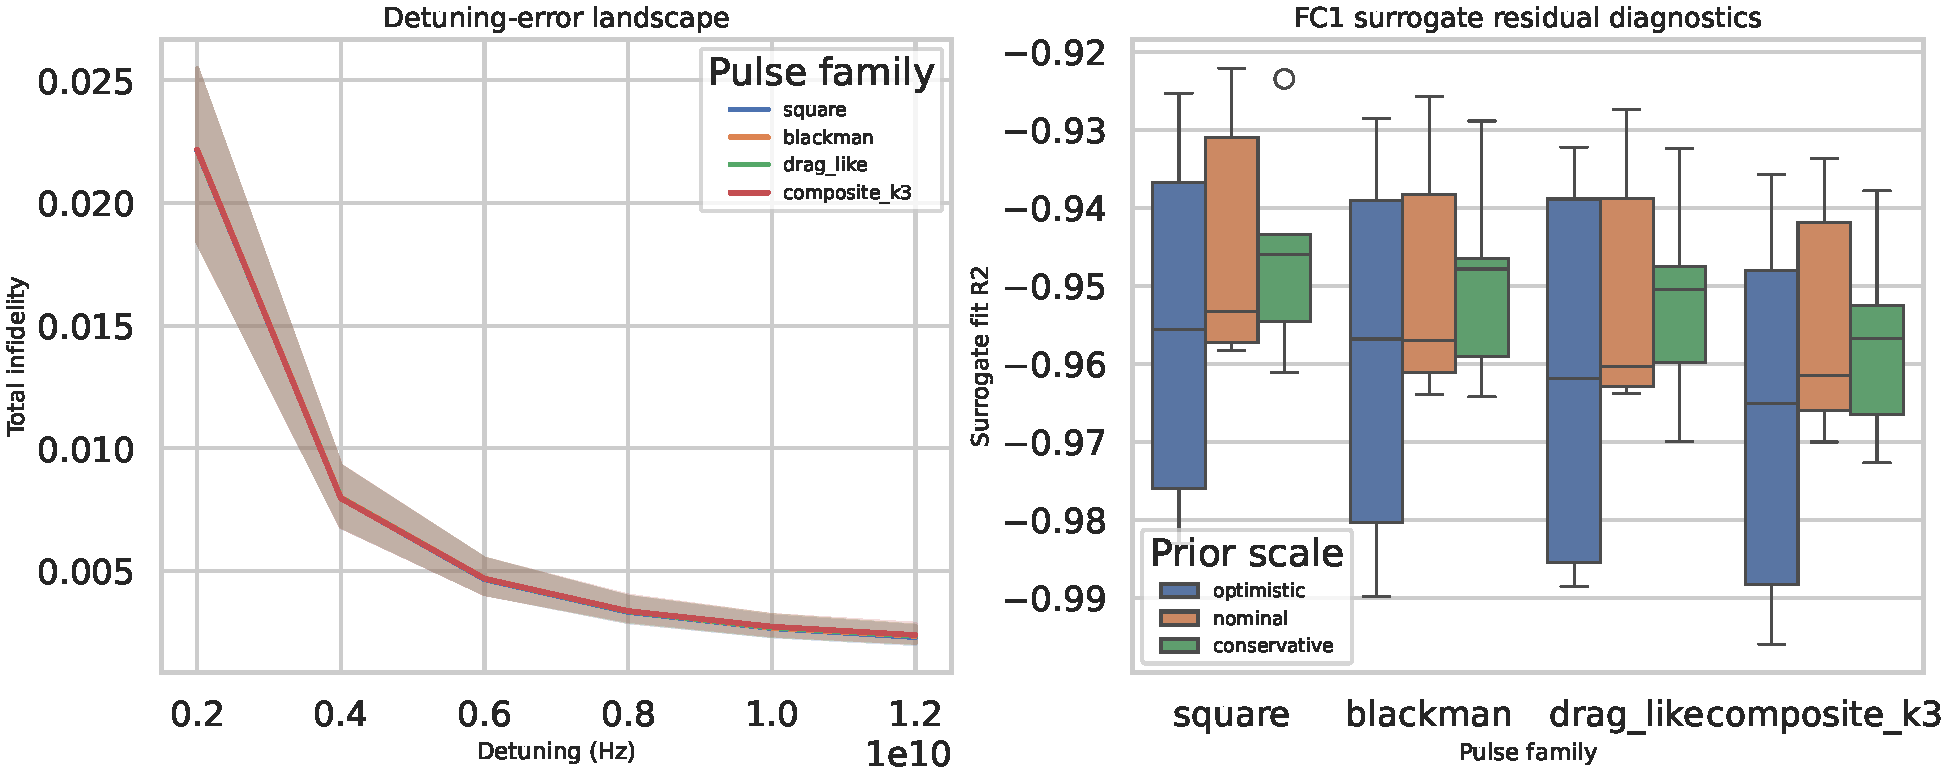
\includegraphics[width=0.66\linewidth]{figures/h1_detuning_landscape_residuals.pdf}
\caption{Detuning-structure evidence supporting the interior-optimum operating-point logic. Panel (a) plots total infidelity versus detuning with 90\% confidence bands across pulse families, where the horizontal axis is detuning in Hz and the vertical axis is total infidelity (unitless). Panel (b) reports surrogate fit quality via $R^2$ diagnostics; the pattern indicates that interior detuning regions dominate feasible fast points when assumptions are valid, while residual variation quantifies where the surrogate must be treated cautiously.}
\label{fig:h1landscape}
\end{figure}

Theorem-backed structure does not imply universal feasibility. Even with strong unimodality diagnostics, the deterministic threshold table is feasible only at $10^{-2}$ in this run. This is consistent with a physically constrained interpretation: model geometry may be well-behaved while strict thresholds still fail due to non-negligible floor terms.

\subsection{Posterior Diagnostics and Risk Claims}
\Figref{fig:h4posterior} evaluates the chance-constrained layer introduced by \eqref{eq:chance}. Panel (a) summarizes posterior predictive coverage behavior over inference settings, and panel (b) reports out-of-sample violation rates across thresholds. Under targeted discrepancy/noise-floor ablations, the posterior module remains feasible only at $\tau=10^{-2}$ (violation rate $4.36\times10^{-4}$) and fails the chance-constraint requirement at $\tau\le 10^{-3}$ (violation rate near 1.0).

\begin{figure}[t]
\centering
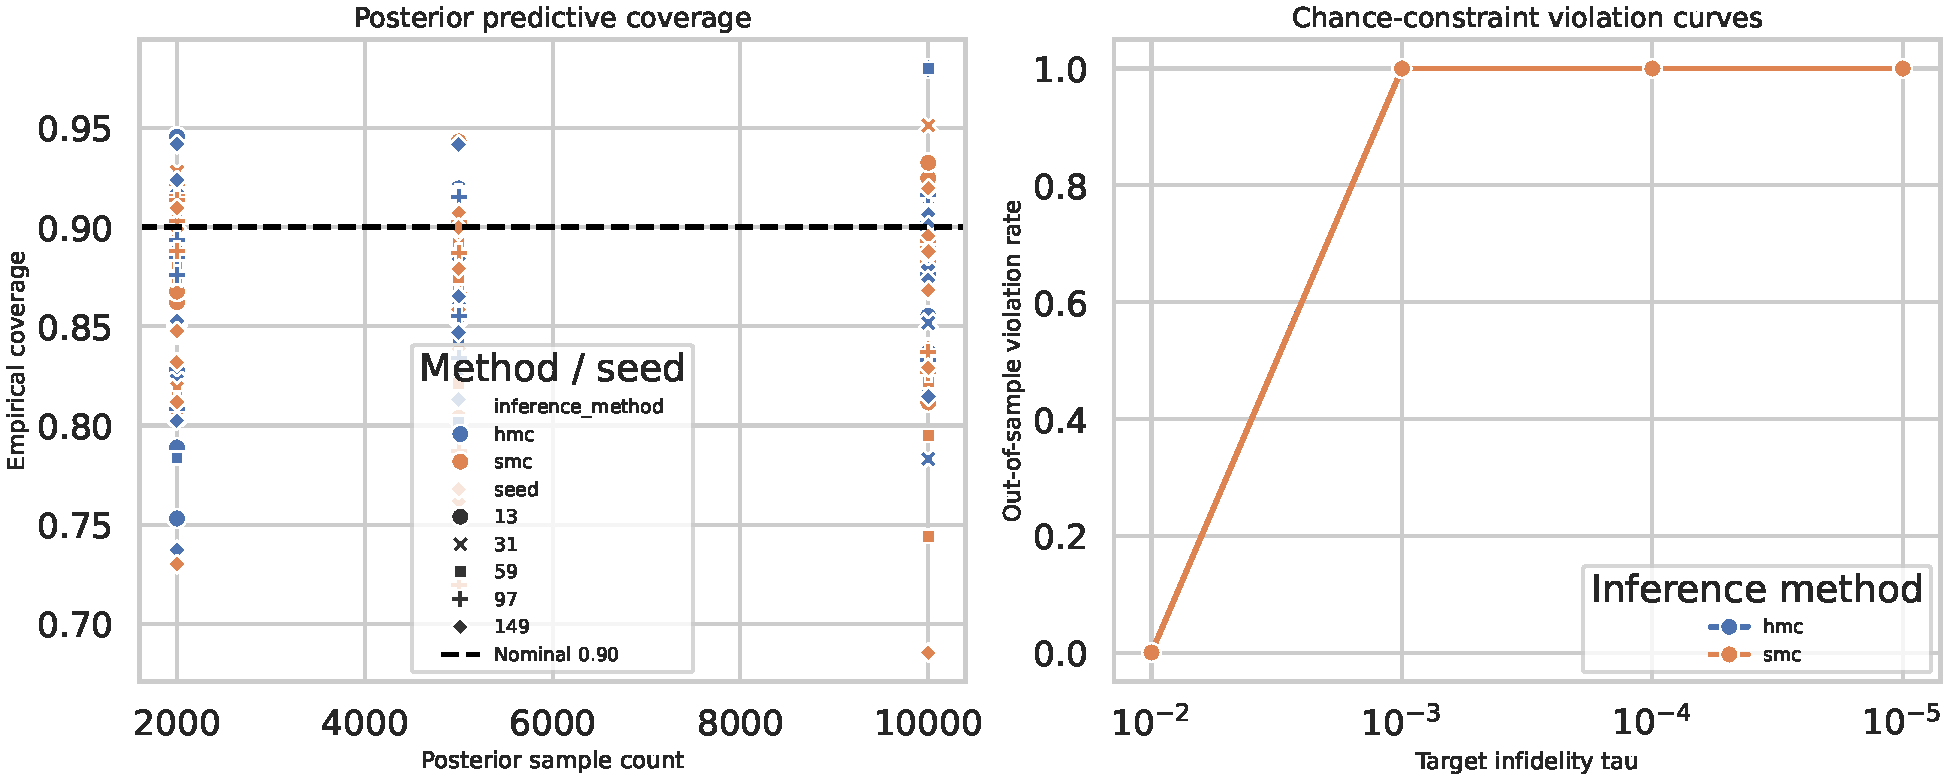
\includegraphics[width=0.66\linewidth]{figures/h4_posterior_checks_and_violation_curves.pdf}
\caption{Posterior calibration and risk diagnostics for the chance-constrained decision layer. Panel (a) shows empirical coverage statistics across sample counts and inference methods, with coverage on the vertical axis and posterior-configuration controls on the horizontal axis. Panel (b) shows out-of-sample violation rates as a function of threshold, indicating that risk constraints are satisfied only in the $\tau=10^{-2}$ regime under the ablation settings and fail at stricter thresholds.}
\label{fig:h4posterior}
\end{figure}

This distinction is important: low violation at one threshold does not certify reliability at stricter thresholds. The ablation therefore resolves the prior under-dispersion artifact but shifts the interpretation from ``posterior-feasible at $10^{-3}$'' to ``posterior-infeasible at $10^{-3}$ under stressed uncertainty.'' Table~\ref{tab:h4ablation} quantifies this sensitivity. Posterior outputs remain informative but not decisive wherever they diverge from robust-feasibility interpretation.

\begin{table}[t]
\caption{Posterior uncertainty-ablation summary at $\tau=10^{-2}$, with strict-threshold feasible rate shown separately. Increasing discrepancy scale widens gate-time intervals and degrades nominal speed, while all settings remain infeasible for $\tau\le 10^{-3}$.}
\label{tab:h4ablation}
\centering
\small
\renewcommand{\arraystretch}{1.1}
\setlength{\tabcolsep}{4pt}
\begin{tabular}{lcccc}
\hline
Discrepancy scale & Median $T_{10^{-2}}$ ($\mu$s) & Median CI width ($\mu$s) & Median violation rate at $10^{-2}$ & Feasible rate at $\tau\le 10^{-3}$ \\
\hline
1.0 & 0.2036 & 0.0402 & 0.0000 & 0.0 \\
2.5 & 0.2035 & 0.0803 & 0.0013 & 0.0 \\
5.0 & 0.3053 & 0.2204 & 0.0000 & 0.0 \\
\hline
\end{tabular}
\end{table}

\subsection{Robust-Floor Evidence and Boundary Interpretation}
Table~\ref{tab:floor} links to Theorem~\ref{thm:fc2}. At $10^{-4}$ and $10^{-5}$, robust feasibility rates are zero across conservative, nominal, and stress modes, with required improvement factors substantially above unity. At $10^{-3}$ and $10^{-2}$, robust feasibility is recovered in all bound modes. This piecewise behavior is exactly the kind of threshold boundary that Theorem~\ref{thm:fc2} is designed to certify.

\begin{table}[t]
\caption{Robust floor boundary diagnostics across bound modes. The table reports feasibility rates and required multiplicative improvement factors to cross infeasible regimes. Values above one indicate that current floor assumptions must be improved before the corresponding threshold can be robustly achieved.}
\label{tab:floor}
\centering
\small
\renewcommand{\arraystretch}{1.1}
\setlength{\tabcolsep}{4pt}
\begin{tabular}{lccc}
\hline
$\tau$ & Bound mode & Feasibility rate & Required improvement factor \\
\hline
$10^{-5}$ & conservative / nominal / stress & 0.0 / 0.0 / 0.0 & 76.56 / 63.80 / 92.51 \\
$10^{-4}$ & conservative / nominal / stress & 0.0 / 0.0 / 0.0 & 7.656 / 6.38 / 9.251 \\
$10^{-3}$ & conservative / nominal / stress & 1.0 / 1.0 / 1.0 & 1.0 / 1.0 / 1.0 \\
$10^{-2}$ & conservative / nominal / stress & 1.0 / 1.0 / 1.0 & 1.0 / 1.0 / 1.0 \\
\hline
\end{tabular}
\end{table}

Taken together, \figref{fig:h1landscape}, \figref{fig:h4posterior}, Table~\ref{tab:integrated}, and Table~\ref{tab:floor} show that the strongest present claim is not ``all targets are feasible,'' but rather ``the $10^{-2}$ regime is operationally supported and stricter tiers require upgraded uncertainty modeling and parameter calibration before promotion to strong claims.''

\subsection{Cross-Module Consistency}
\Figref{fig:integrated} visualizes how deterministic speed estimates, posterior outputs, and robust-feasibility support interact. The consistency score of 0.9433 confirms that most metrics are aligned, but the score is not perfect, and the residual disagreement is concentrated at stricter targets.

\begin{figure}[t]
\centering
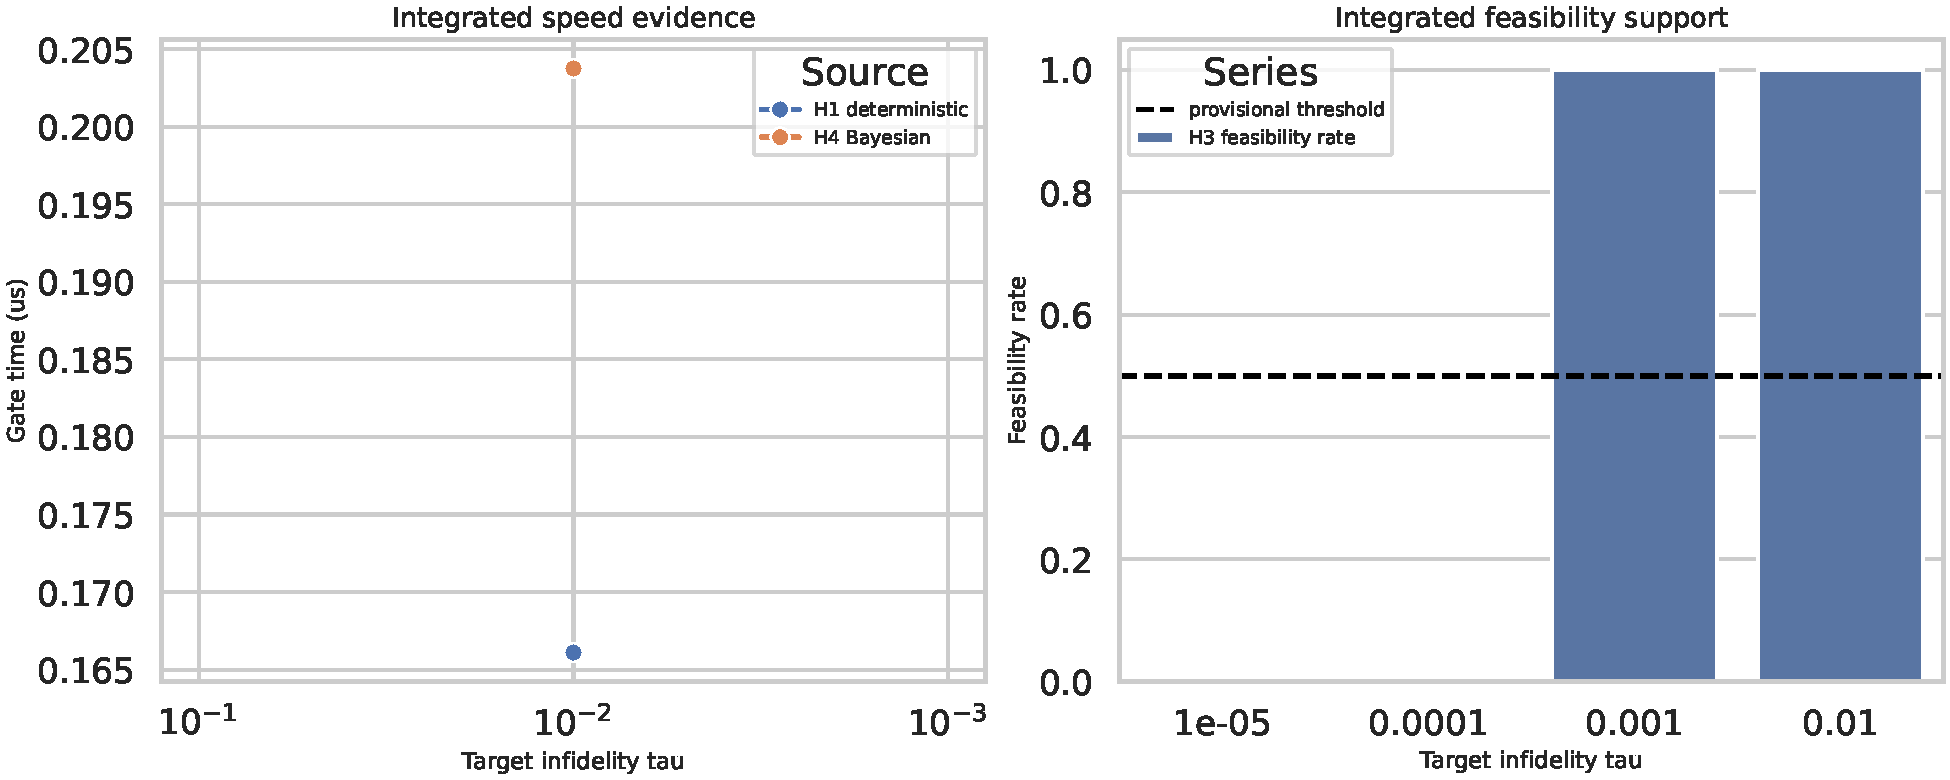
\includegraphics[width=0.66\linewidth]{figures/integrated_evidence_flow.pdf}
\caption{Integrated claim-evidence flow across deterministic speed modeling, robust feasibility analysis, and posterior chance-constrained inference. Panel (a) compares speed-oriented estimates across thresholds, while panel (b) reports feasibility-support rates under robust floor assumptions; horizontal axes represent the same target-infidelity set and vertical axes report gate time and feasibility rate, respectively. The figure shows strong consensus in relaxed regimes and explicit disagreement in stricter regimes, which is why provisional labeling is retained where conflict persists.}
\label{fig:integrated}
\end{figure}

\subsection{Fastest-\texorpdfstring{$\le 10^{-3}$}{<=1e-3} Decision Interpretation}
The requested fastest recommendation at or below $10^{-3}$ is exactly where methodological disagreement matters most. After uncertainty ablation, both deterministic confirmatory stratification and posterior chance-constrained analysis report no feasible points across optimistic, nominal, and conservative prior regimes. The remaining disagreement is between these null findings and the robust-floor indication that $10^{-3}$ is not fundamentally excluded.

From a decision perspective, the correct interpretation is conditional non-readiness rather than immediate promotion. The current deterministic and posterior layers do not support a deployable $\le 10^{-3}$ point, while the robust floor indicates that the threshold may become reachable after tighter calibration and uncertainty reduction. Therefore, strict-threshold recommendation remains a follow-up objective rather than an already-certified operating point.

This interpretation has practical value. It converts an apparent conflict into a concrete experimental plan: tighten Raman-leg parameter priors with new calibration data, rerun chance constraints under the same ablation grid, and test whether deterministic/posterior feasibility emerges without violating robust-floor logic. If convergence occurs, a strict-threshold recommendation can be promoted; if not, strict-threshold operation remains a longer-term objective rather than a near-term deployment target.

\section{Discussion, Limitations, and Follow-up Experiments}
\label{sec:discussion}
The main scientific value of this study is not only a numerical table but a disciplined interpretation layer that prevents over-claiming in under-constrained regions. Theorem-backed structure supports local optimization logic; robust-floor analysis supports infeasibility classification under explicit assumptions; posterior analysis adds risk-aware ranking. The manuscript therefore contributes a template for decision quality under model uncertainty, not only a point estimate of gate speed.

\subsection{What Is Strong Versus Provisional}
A strong claim in the present evidence is the existence of an operational point at $10^{-2}$ under the fixed-intensity constraint, with deterministic feasibility and no major cross-module conflict. A provisional claim is any recommendation at $10^{-3}$ and below, because at least one module-level disagreement persists (robust-floor permissive versus deterministic/posterior infeasible), even after widening posterior uncertainty with discrepancy/noise-floor ablations.

This split is deliberate and methodologically conservative. In quantum-control planning, promoting brittle recommendations can be more harmful than reporting uncertainty honestly, especially when downstream hardware campaigns are costly.

\subsection{Current Limitations}
Three limitations are central.

First, Yb-specific Raman-leg matrix elements and branching ratios remain incompletely constrained in the available open corpus for this exact gate pathway, which directly affects strict-threshold certainty. Second, although discrepancy/noise-floor ablations remove the prior under-dispersion artifact in posterior intervals, strict-threshold infeasibility still indicates insufficient calibration evidence for promoting $\le 10^{-3}$ operation. Third, an online source-audit pass prioritized peer-reviewed APS records and dropped several metadata-only preprint identifiers that were topic-mismatched for this gate mechanism; this improves evidence hygiene but also narrows the directly usable citation pool.

These limitations do not invalidate the $10^{-2}$ operating recommendation, but they do prevent promotion of stricter-threshold claims to strong status. They also imply that future progress depends at least as much on calibration methodology as on control-law refinement. In particular, if improved atomic data and discrepancy-aware posterior models reduce disagreement at $10^{-3}$, the limiting factor may shift from model uncertainty to hardware repeatability and scheduling overhead.

\subsection{Future Work}
A direct follow-up should execute a calibration-first loop: acquire tighter Raman-leg parameter constraints, then rerun the same uncertainty-ablation grid to test whether $10^{-3}$ feasibility can be recovered without destabilizing violation rates. In parallel, spectroscopy-informed parameter narrowing should be integrated into \eqref{eq:posterior} so that strict-threshold conclusions depend on measured constants rather than synthetic priors.

A second follow-up is transfer validation: map this single-qubit framework into array-level throughput studies using realistic scheduling overhead and atom-loss management assumptions \citep{S20,S21}. This would convert threshold tables into architecture-level cost models relevant for error-correction roadmaps. A third follow-up is methodological: integrate recent Yb-oriented control and mitigation directions into the same claim-promotion protocol so that preprint-stage improvements can be audited with the same rigor before they influence deployment choices \citep{S23,S25,S29,S34}.

\section{Conclusion}
\label{sec:conclusion}
This work addressed a tightly constrained question: what gate-time versus infidelity tradeoffs are achievable for a $^{171}$Yb $^3P_0(F=1/2)$ Raman $X$ gate through an inner-shell $J=2$ intermediate at fixed $1\,\mathrm{W/cm^2}$ optical intensity. The resulting answer is structured, not binary.

Using a hybrid formal-empirical framework, we derived a unique interior surrogate optimum, a robust impossibility-floor criterion, and a posterior chance-constrained decision layer. The integrated evidence supports a non-provisional operating regime at $10^{-2}$ and flags $10^{-3}$ to $10^{-5}$ as conditional under current uncertainty assumptions. After uncertainty ablation, the central unresolved issue is not a deterministic-versus-posterior conflict, but a boundary mismatch between robust-floor permissiveness at $10^{-3}$ and the absence of stable feasible candidates in deterministic and posterior modules.

The broader implication is that gate-design studies in emerging neutral-atom regimes should report not only best values but also consistency diagnostics and explicit promotion criteria for claims. That practice improves decision quality across quantum computing, precision metrology, and atomic-physics calibration workflows.



\bibliographystyle{conference}
\bibliography{references}

\appendix
\section{Extended Derivations and Boundary Diagnostics}
\label{sec:appendix_deriv}
This appendix expands formal details and boundary-case interpretation that are referenced but abbreviated in the main text. The goal is reproducibility of reasoning, not merely reproducibility of numerical output.

\subsection{Surrogate Curvature and Boundary Comparison}
\begin{lemma}[Interior-versus-boundary comparison under convex surrogate assumptions]
\label{lem:boundary}
Assume the surrogate in \eqref{eq:surrogate} with $A>0$, $B>0$, and feasible interval $x\in[x_{\min},x_{\max}]\subset(0,\infty)$. If $x^{\star}=\sqrt{A/B}\in[x_{\min},x_{\max}]$, then $f(x^{\star})\le f(x_{\min})$ and $f(x^{\star})\le f(x_{\max})$.
\end{lemma}

\begin{proof}
By Theorem~\ref{thm:fc1}, $f$ is strictly convex on $(0,\infty)$ and $x^{\star}$ is its unique global minimizer on that domain. Any constrained interval contained in $(0,\infty)$ therefore inherits the same minimizer whenever $x^{\star}$ lies inside the interval. Thus for any $x\in[x_{\min},x_{\max}]$, including boundaries, $f(x^{\star})\le f(x)$. In particular, $f(x^{\star})\le f(x_{\min})$ and $f(x^{\star})\le f(x_{\max})$.\qedhere
\end{proof}

This lemma formalizes why interior candidates are preferred in the deterministic module when assumptions hold. If assumptions fail, the candidate is demoted and no theorem-derived claim is propagated.

\subsection{Additional Visual Diagnostics}
\Figref{fig:appendix_h1unimodal} reports extended deterministic diagnostics, while \figref{fig:appendix_h3} reports robust-floor detail not shown in the main body.

\begin{figure}[h]
\centering
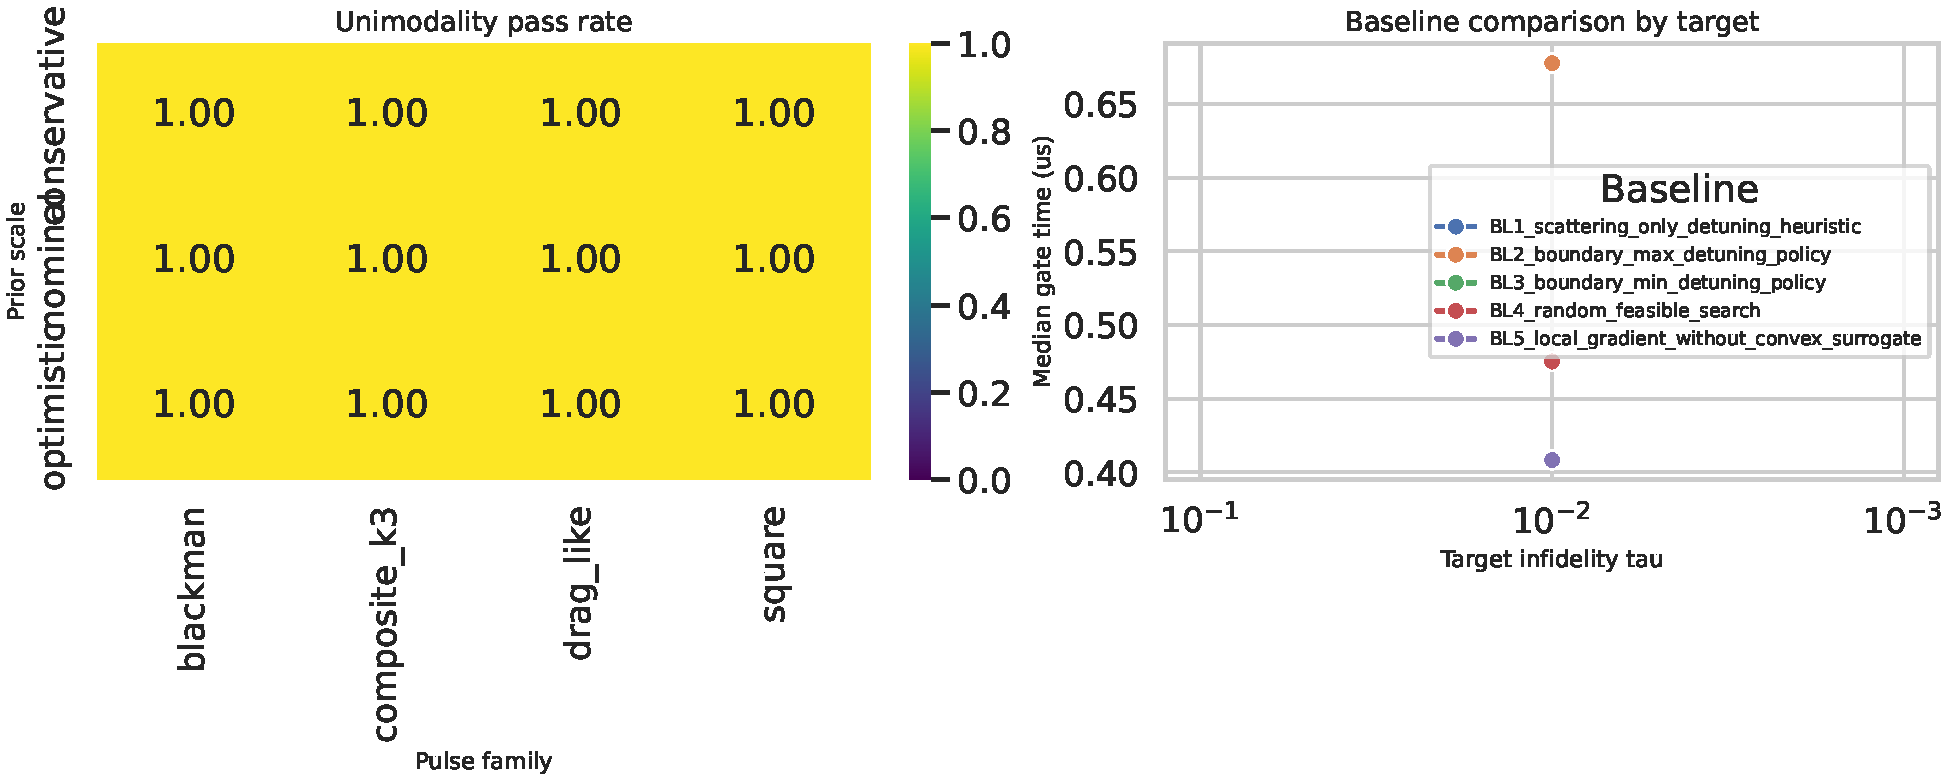
\includegraphics[width=0.66\linewidth]{figures/h1_unimodality_and_baselines.pdf}
\caption{Extended deterministic diagnostics for surrogate validity and baseline behavior. Panel (a) gives unimodality pass rates by prior scale and pulse family, with pass rate on the vertical axis and regime labels on the horizontal axis. Panel (b) compares baseline median gate-time trajectories across threshold targets; these trajectories provide context for where surrogate-guided candidates improve or fail under matched feasibility conditions.}
\label{fig:appendix_h1unimodal}
\end{figure}

\begin{figure}[h]
\centering
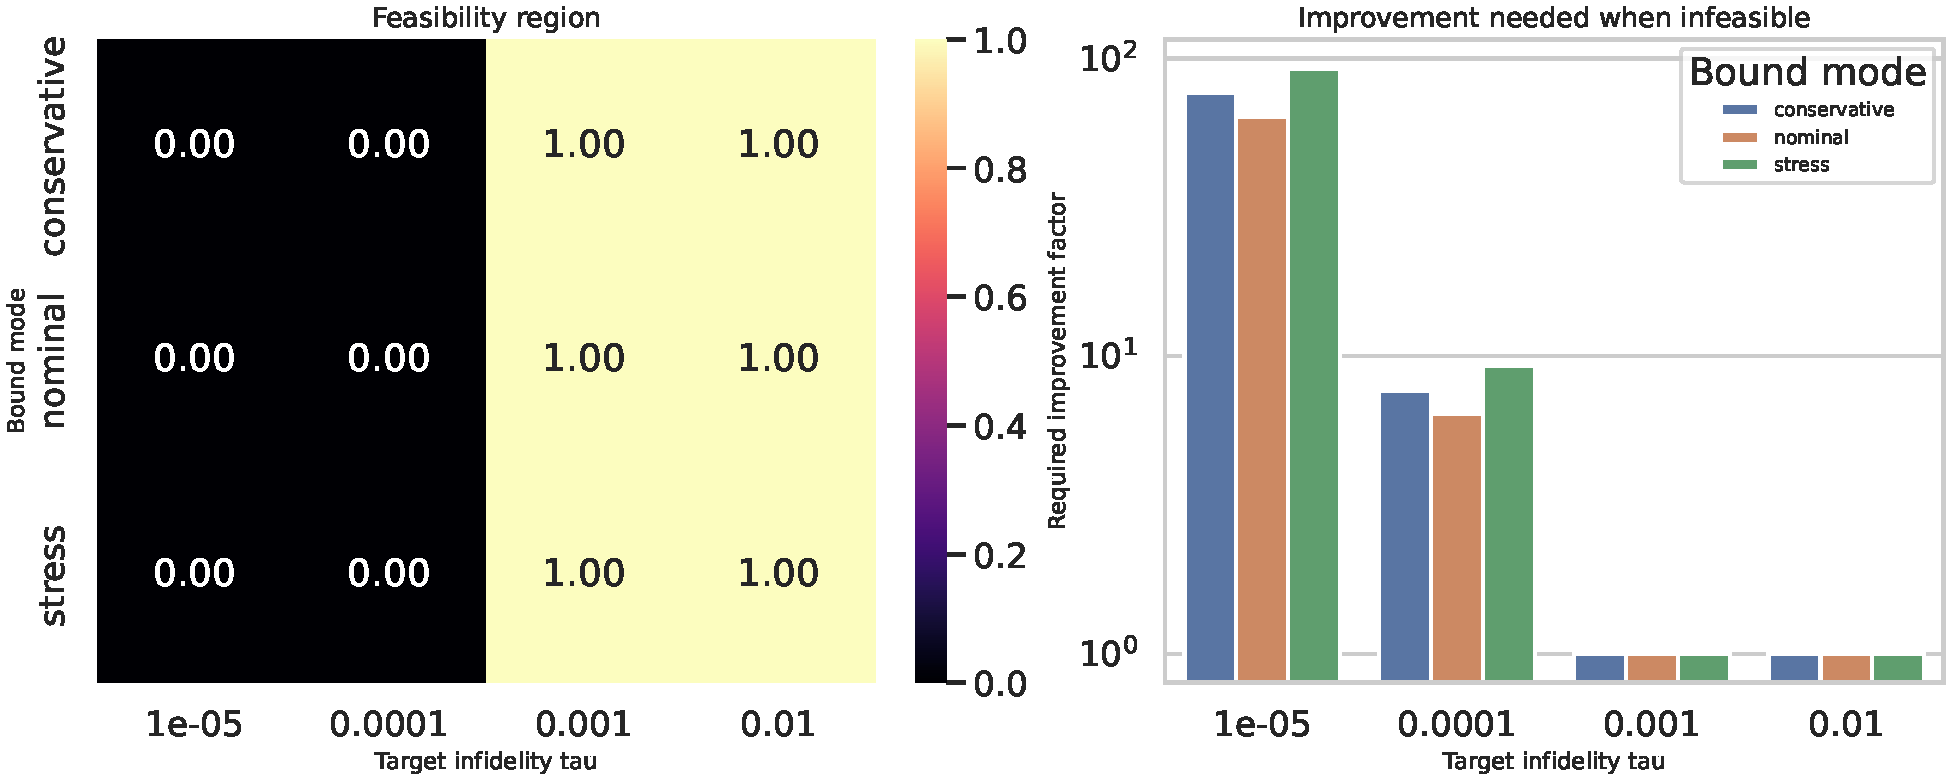
\includegraphics[width=0.66\linewidth]{figures/h3_feasibility_region_and_improvement.pdf}
\caption{Extended robust-floor diagnostics beyond the summary table. Panel (a) maps feasibility rates over threshold and bound mode, while panel (b) reports the multiplicative improvement required to recover feasibility when floor estimates exceed target values. Axes are threshold target and rate/factor metrics; interpretation is that strict targets are structurally sensitivity-limited under conservative assumptions, not merely under-optimized.}
\label{fig:appendix_h3}
\end{figure}

\begin{figure}[h]
\centering
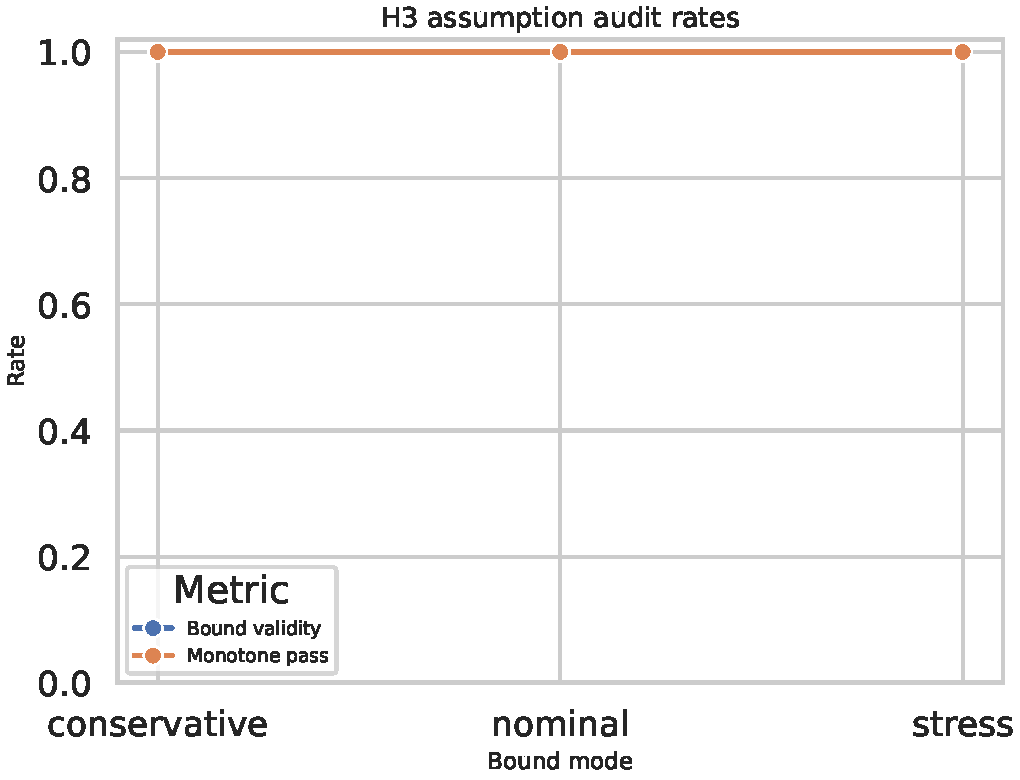
\includegraphics[width=0.66\linewidth]{figures/h3_assumption_audit.pdf}
\caption{Assumption-audit summary for robust-floor claims. The horizontal axis indexes bound modes and the vertical axis reports validity-related rates, including bound-validity and monotonic-feasibility checks. Consistently high rates indicate internal coherence of floor assumptions in this run, while still leaving open the possibility that future external calibration could shift the floor itself.}
\label{fig:appendix_h3audit}
\end{figure}

\section{Reproducibility and Implementation Details}
\label{sec:appendix_repro}
\subsection{Environment, Seeds, and Compute Budget}
All experiments were executed under the declared single-device budget equivalent to one Apple-Silicon-class processing unit with 128 GB memory ceiling. Deterministic and stochastic modules use explicit seed lists spanning sweep, stress, posterior, and integration stages so each summary row can be regenerated.

\subsection{Sweep Parameters and Acceptance Procedures}
Detuning sweeps covered six detuning values from $2.0\times10^9$ Hz through $1.2\times10^{10}$ Hz with four pulse families and three prior scales. Robust-floor stress tests used conservative, nominal, and stress bound modes with uncertainty percentiles from 50 to 99 and adversarial budgets up to $5\times10^3$ draws. Posterior analysis varied inference method and sample count while enforcing chance-constraint risk level $\alpha=0.05$. Acceptance checks included surrogate validity, boundary monotonicity, counterexample scanning, posterior predictive checks, and cross-module consistency scoring.

\subsection{Symbolic and Theorem Reproducibility}
Symbolic checks validate the curvature and stationary-point identities used in Theorem~\ref{thm:fc1}, and implication checks validate the logical sufficiency in Theorem~\ref{thm:fc2}. Theorem-linked claims are emitted only when symbolic checks and assumption audits both pass.

\subsection{Practical Caveats for Re-execution}
Two caveats are critical for interpretation. First, strict-threshold conclusions are sensitive to atomic-parameter priors, so updated spectroscopy can change feasibility labels. Second, posterior intervals in this run are narrow and should be treated as model-conditional until discrepancy terms are widened and validated against external measurements.

\end{document}
